\usetikzlibrary{arrows.meta, positioning}

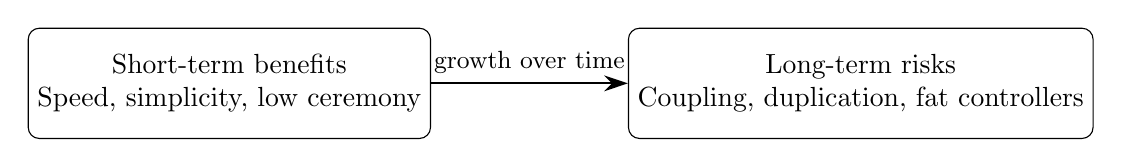
\begin{tikzpicture}[
    node distance=2.0cm and 2.5cm,
    box/.style={draw, rounded corners, align=center, minimum width=4.8cm, minimum height=1.4cm},
    arrow/.style={-{Stealth[length=3mm, width=2mm]}, thick}
]
    \node[box] (pros) {Short-term benefits\\Speed, simplicity, low ceremony};
    \node[box, right=of pros] (cons) {Long-term risks\\Coupling, duplication, fat controllers};

    \draw[arrow] (pros.east) -- node[above, font=\small] {growth over time} (cons.west);
\end{tikzpicture}
